% -----------------------------------------------------------------------------
\section{Example of Data Model}
\label{sec:examples}
% -----------------------------------------------------------------------------

%\subsection{LacI/TetR Toggle Switch}

This section illustrates how to use the SBOL data model by specifying the design of a LacI/TetR toggle switch similar to those constructed in \cite{Gardner2000}. This design is visualized in \ref{images:toggleswitch_modular}. 

\begin{figure}[ht]
\begin{center}
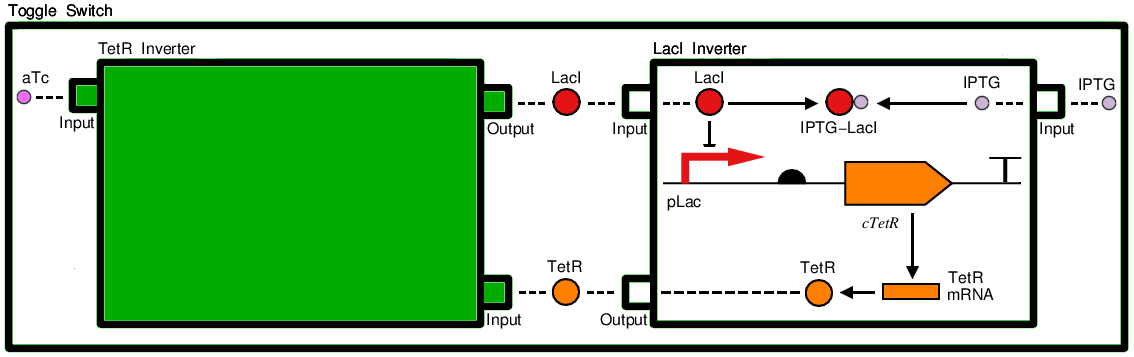
\includegraphics[scale=0.4]{images/toggleswitch_modular}
\caption[]{Design of a LacI/TetR toggle switch. This design is composed of two inverter sub-designs, each containing a single gene. These genes mutually repress each other's expression via their encoded protein transcription factors, LacI and TetR. Furthermore, both LacI and TetR are bound by specific small molecules that sequester them and prevent them from acting as repressors. In this design, arrows represent different molecular interactions, including the repression of pLac via LacI, the non-covalent binding of IPTG to LacI, the transcription of TetR mRNA, and the translation of TetR. Dashed lines serve to map between transcription factors in the inverter sub-designs and those in the overall toggle switch design.}
\label{images:toggleswitch_modular}
\end{center}
\end{figure}

The LacI/TetR toggle switch is modeled in SBOL as two parallel hierarchies of structure and function. Structurally, \sbol{ComponentDefinition} objects are used to hierarchically define the physical elements that comprise the toggle switch:
\begin{itemize}
\item The base elements of the hierarchy are genetic elements, transcription factor complexes, and small-molecules.  As examples, \ref{uml:ex_comp_defs} shows UML diagrams of a number of such \sbol{ComponentDefinition} objects.
\item These are composed to form more complex structures such as multi-element genetic complexes and molecular complexes. As examples, \ref{uml:ex_comp_def_compo} shows UML diagrams of the composite \sbol{ComponentDefinition} for the DNA construct for regulated expression of TetR and for the IPTG-LacI complex.
\end{itemize}

\begin{figure}[ht]
\begin{center}
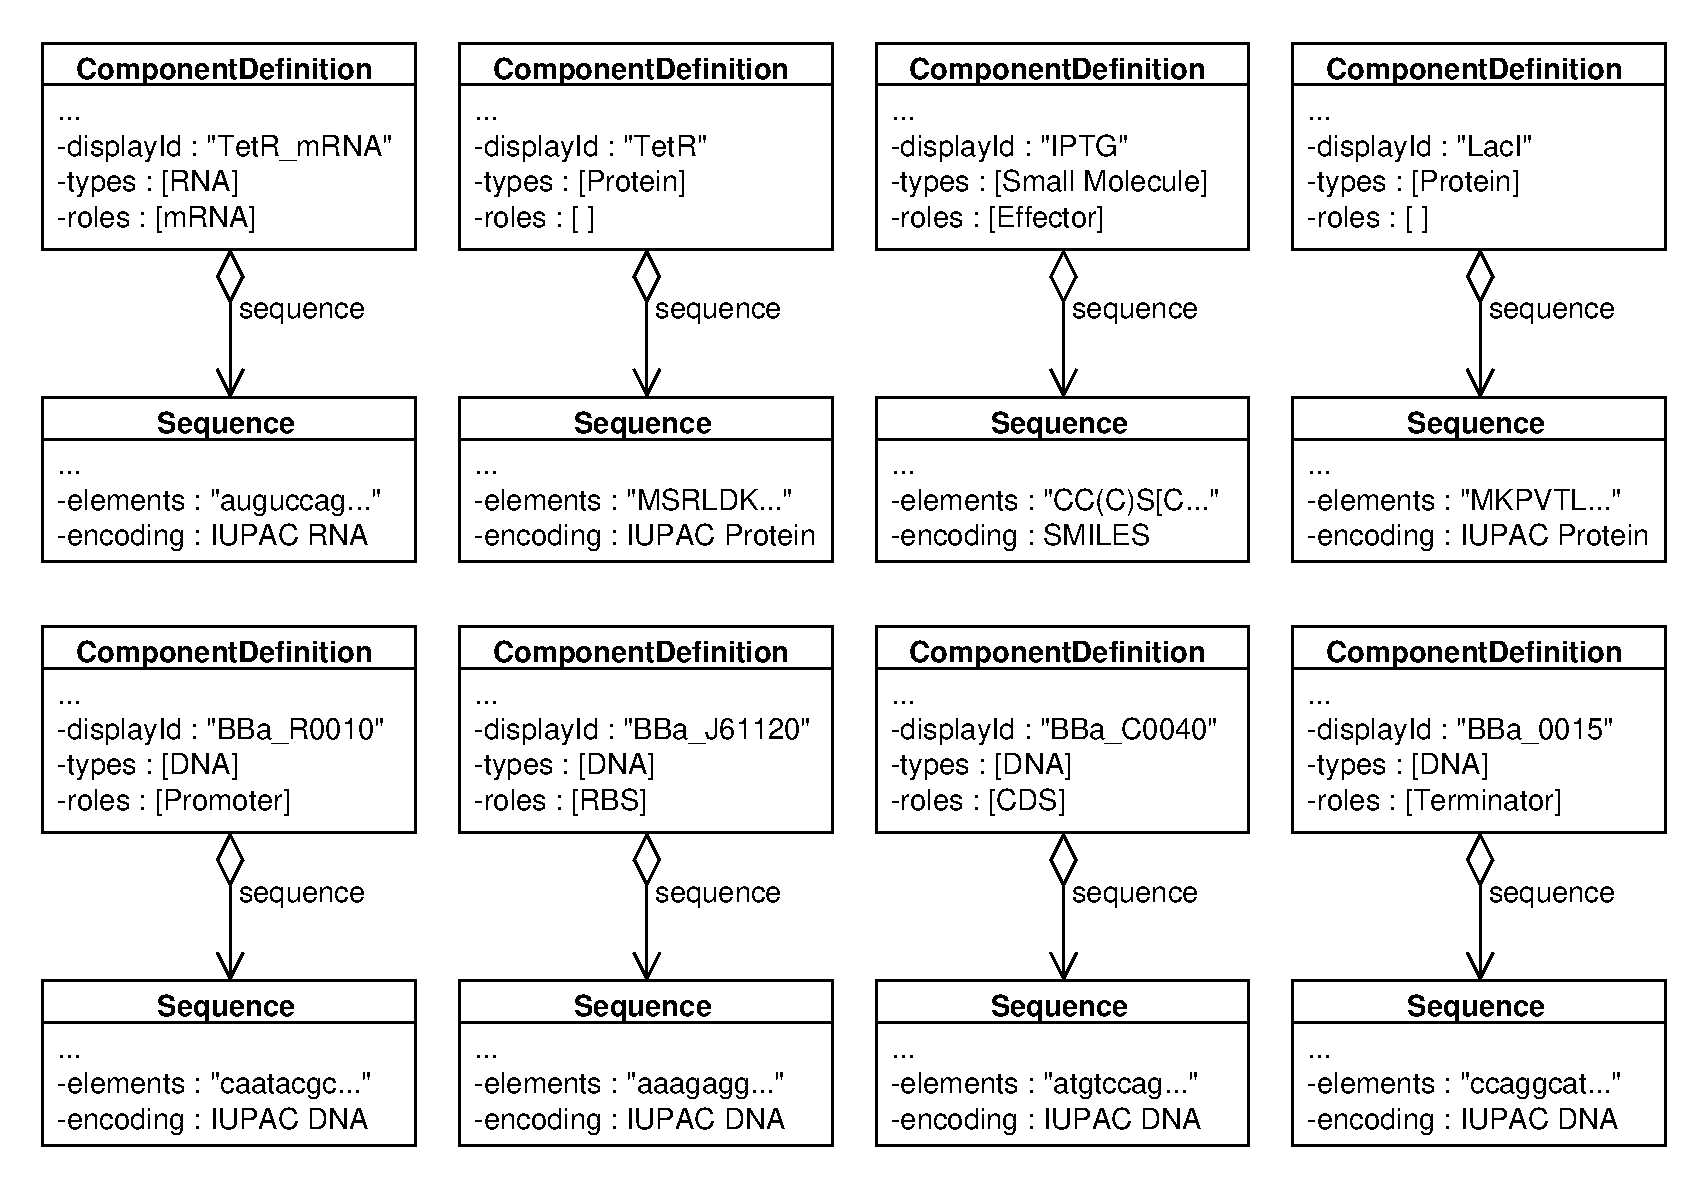
\includegraphics[width=\textwidth]{example_uml/toggle_1}
\caption[]{Examples of component definitions for the LacI inverter. These include DNA \sbol{ComponentDefinition}s based on parts from the iGEM Registry, the RNA and protein \sbol{ComponentDefinition}s derived from them, and the small molecule \sbol{ComponentDefinition} for IPTG. Each \sbol{ComponentDefinition} in this example is associated with a \sbol{Sequence} that has an IUPAC nucleic acid or amino acid encoding, except the \sbol{ComponentDefinition} for IPTG, which is associated with a \sbol{Sequence} that has a SMILES encoding.}
\label{uml:ex_comp_defs}
\end{center}
\end{figure}

\begin{figure}[ht]
\begin{center}
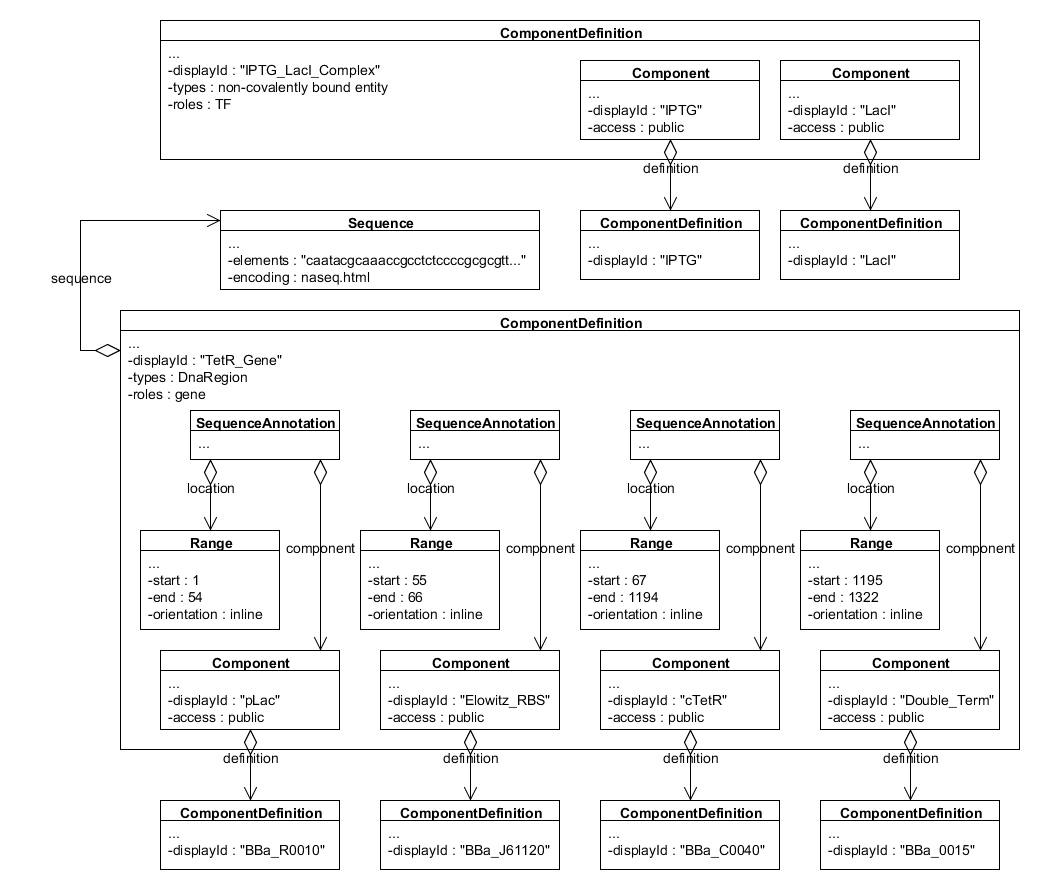
\includegraphics[width=\textwidth]{example_uml/toggle_2}
\caption[]{Example of composite \sbol{ComponentDefinition}s for the LacI inverter. In the case of the TetR gene, its sub-\sbol{Component}s are located as \sbol{Range}s along its \sbol{Sequence} using \sbol{SequenceAnnotation}s. The IPTG-LacI complex, however, has no sequence and its subcomponents are aggregated without any data about their relative locations.}
\label{uml:ex_comp_def_compo}
\end{center}
\end{figure}

The functional hierarchy of the toggle switch is specified using
\sbol{ModuleDefinition} objects:
\begin{itemize}
\item The base elements of the hierarchy are LacI-dependent repression of TetR expression (the LacI inverter) and TetR-dependent repression of LacI (the TetR inverter).  As an example, \ref{uml:ex_mod_def} shows a UML diagram of the LacI inverter module.
\item These are composed as \sbol{Module} objects within the \sbol{ModuleDefinition} for the entire toggle switch.  \ref{uml:ex_mod_def_compo} shows the UML diagram of this composition into the toggle switch.
\end{itemize}

Each \sbol{ModuleDefinition} also contains the \sbol{FunctionalComponent}s that participate in \sbol{Interaction}s and are defined by the same \sbol{ComponentDefinition}s as the parallel \sbol{Component}s in the structural hierarchy of the toggle switch. Finally, \sbol{MapsTo} entities are used to refine which \sbol{FunctionalComponent}s of the functional hierarchy are identical or map them to \sbol{Component}s in the structural hierarchy.
\todo[inline]{Need to clarify this explanation -JSB}

\todo[inline]{ComponentDefinition.types in the following figure are not consistent with the list of BioPax ontological terms described previously in the Data Model section}

As an example of functional representation, \ref{uml:ex_mod_def} specifies the module definition for a LacI inverter. This module definition aggregates and instantiates the component definitions for the TetR gene as functional components that participate in interactions. Note that the transcription and translation of TetR is represented using a single genetic production interaction that abstracts away the presence of the intermediate TetR mRNA. If this additional detail becomes necessary, then a new module could be created that includes both transcription and translation interactions and a TetR mRNA functional component. Finally, the module definition is also associated with a continuous SBML model from source file LacI\_Inverter.xml.
\todo[inline]{This paragraph and next one need better phrasing -JSB}

\begin{figure}[ht]
\begin{center}
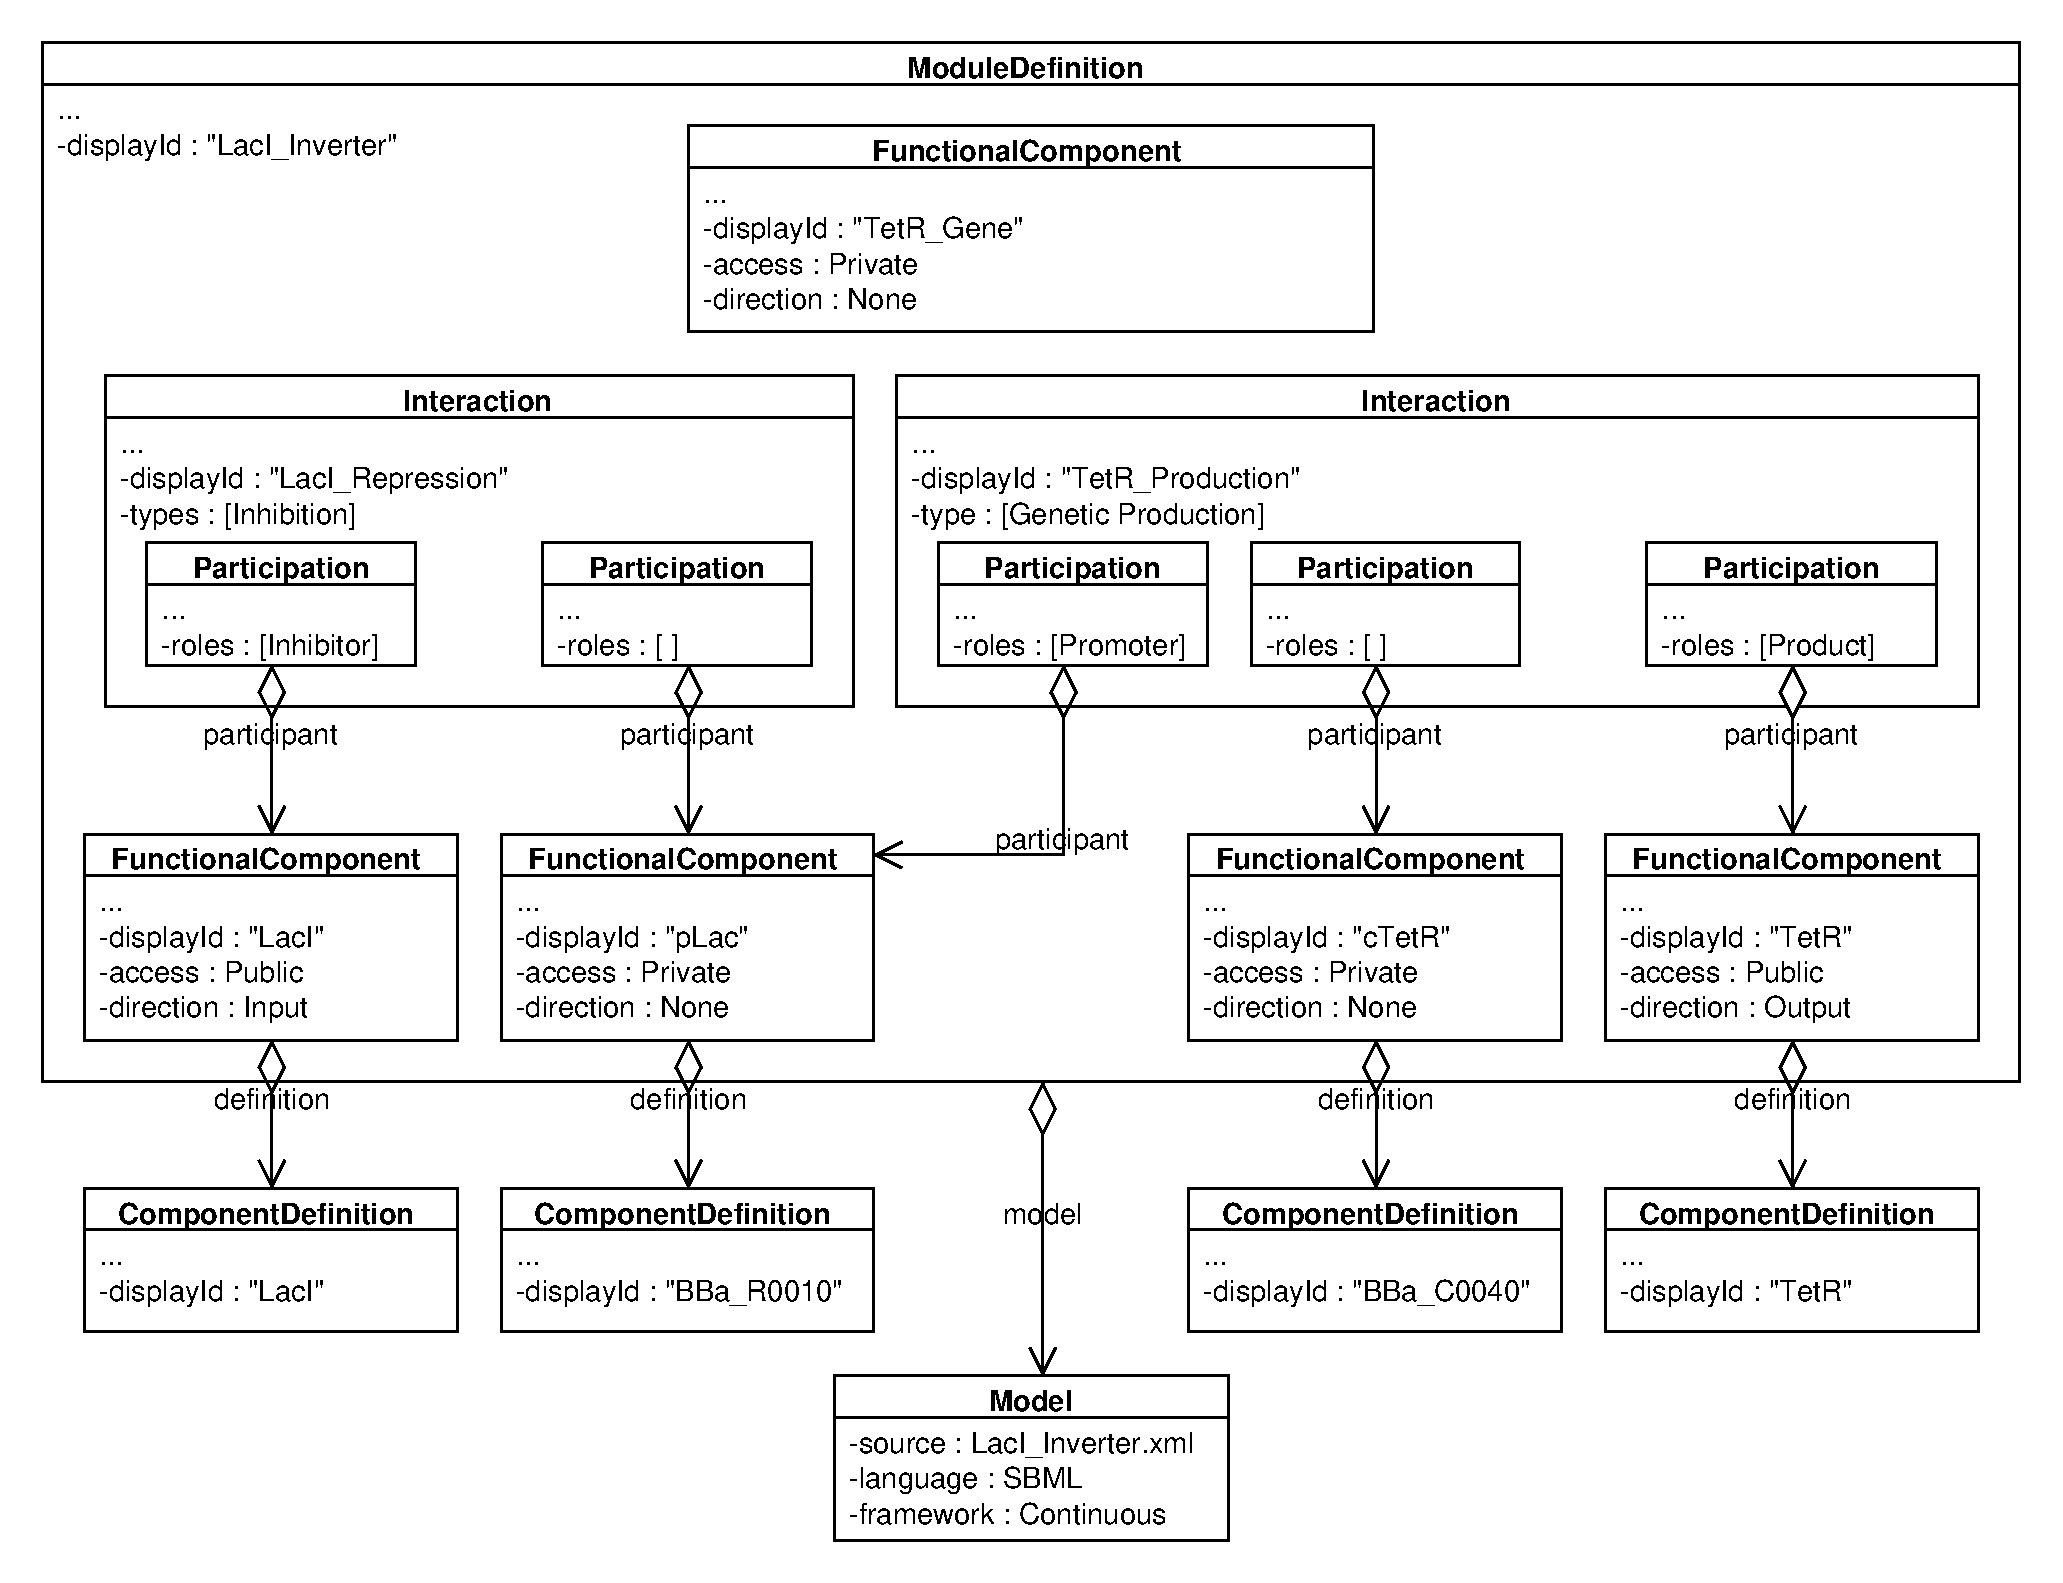
\includegraphics[width=\textwidth]{example_uml/toggle_3}
\caption[]{Example of module definition for a LacI inverter.}
\label{uml:ex_mod_def}
\end{center}
\end{figure}

As an example of functional composition, \ref{uml:ex_mod_def_compo} specifies the composite module definition for the LacI/TetR toggle switch. This module definition aggregates and instantiates the LacI and TetR inverter module definitions as submodules. It also instantiates the LacI and TetR component definitions as the functional component inputs and/or outputs to both the toggle switch and inverter module definitions. To complete the functional composition of the toggle switch, mappings are made between these functional components to indicate that the output of the LacI inverter is the input to the TetR inverter and vice versa.

\begin{figure}[ht]
\begin{center}
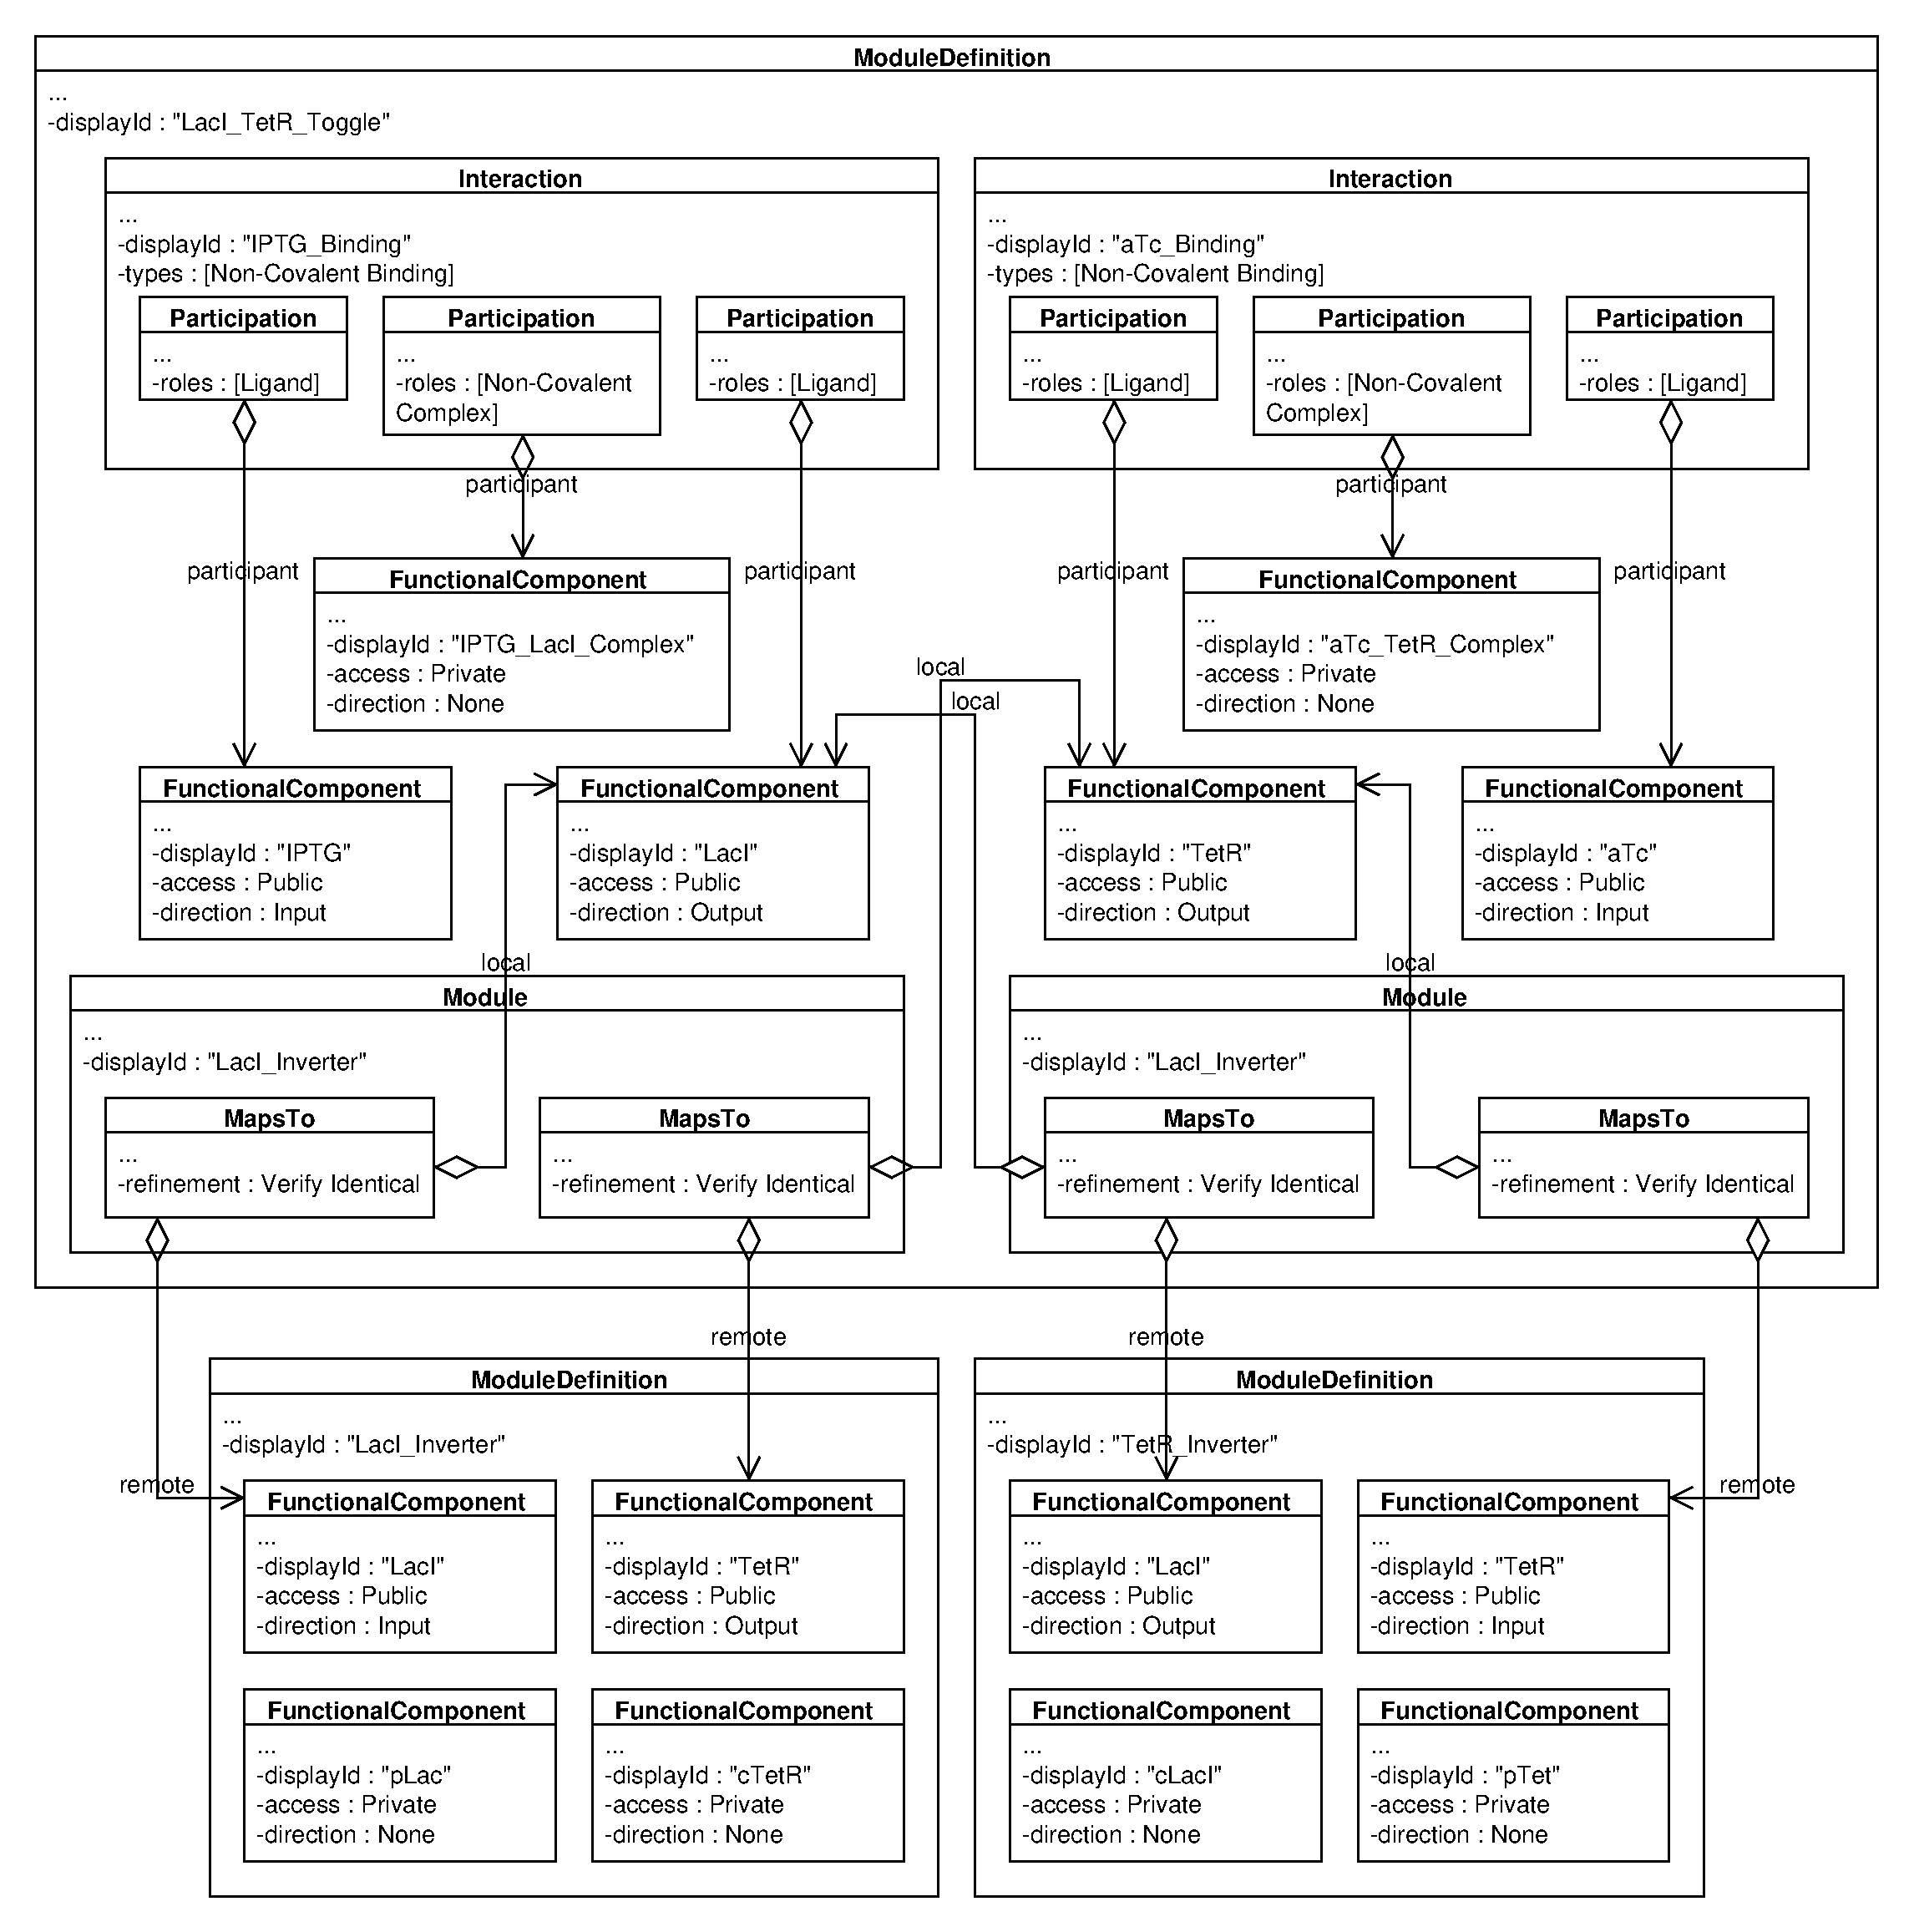
\includegraphics[width=\textwidth]{example_uml/toggle_4}
\caption[]{Example of composing the module definitions for a LacI inverter and TetR inverter into a module definition for a LacI/TetR toggle switch.}
\label{uml:ex_mod_def_compo}
\end{center}
\end{figure}

Lastly, as an example of further detailing the connection between structure and function, \ref{uml:ex_comp_mapping} specifies a mapping between the composite component definition for the TetR gene

%  The first use case is to indicate with greater fidelity how a module describes the function of a composite component, namely by asserting that particular component instantiations within the module correspond to particular component instantiations within the component. 

% As an example of this use case, one might compose the structure and function of the LacI-repressible gene of the genetic toggle switch. In this example, the LacI-repressible gene and two of its subcomponents, the pLac promoter and cTetR CDS, are to be composed with the LacI inverter module. In order to compose these components with the LacI inverter module and indicate that it describes their behavior, they are instantiated inside the module. In addition, port maps are placed on the instantiation of the LacI-repressible gene to connect between its pLac plus cTetR subcomponent instantiations and the corresponding component instantiations in the module. Doing so makes it clear which subcomponent instantiations in the gene are being described by which component instantiations in the module. In this way, GDA tools for sequence editing and biochemical modeling can guarantee that their users are handling corresponding elements of a given genetic design, while GDA tools for genetic technology mapping can make explicit connections between the structural and functional elements of a design.

\begin{figure}[ht]
\begin{center}
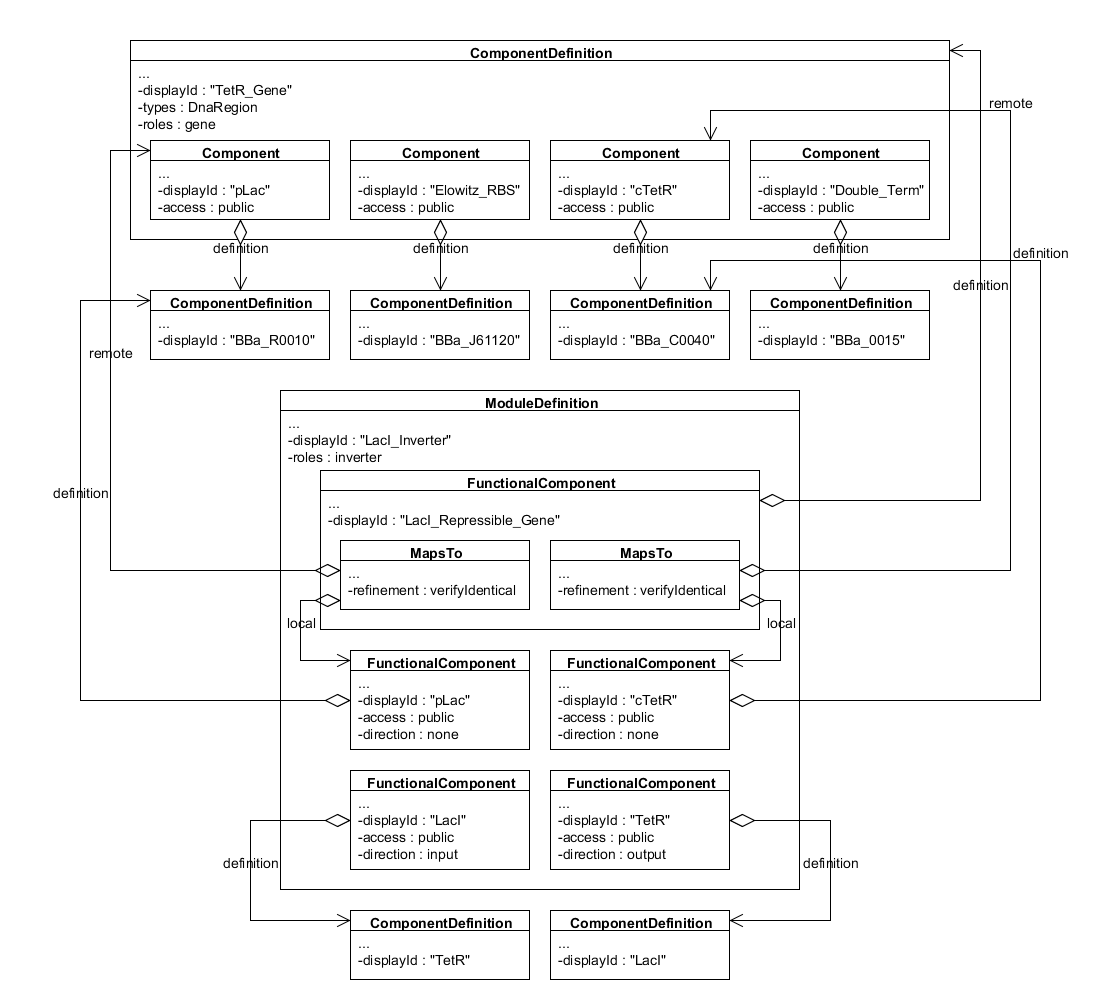
\includegraphics[width=\textwidth]{example_uml/toggle_5}
\caption[]{Example of mapping between the structural and functional components of a LacI inverter.}
\label{uml:ex_comp_mapping}
\end{center}
\end{figure}
